\section{Specifica Back-End}

\subsection{APIMarket::Back-End}

\subsubsection{Informazioni generali}

\begin{figure}[H]
	\centering
	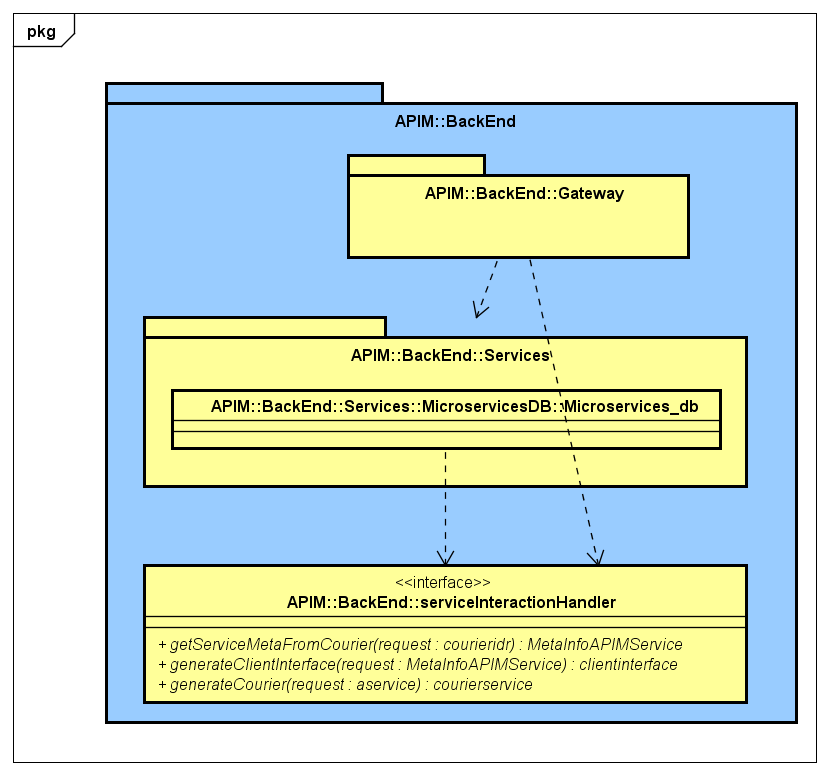
\includegraphics
	[width=0.7\linewidth]
	{UML/DiagrammiPackage/BackEnd.png}
	\caption{Package APIM::BackEnd}
\end{figure}

\begin{itemize}
	\item \textbf{Descrizione:} Il package BackEnd contiene le componenti del lato back-end dell'applicazione web.
	\item \textbf{Packages contenuti:}
	\begin{itemize}
		\item \textbf{Gateway:} package riguardante la gestione delle chiamate ai microservizi.
		\item \textbf{Services:} package riguardante la comunicazione con i database di API Market.
	\end{itemize}
\end{itemize}

\subsubsection{Interfacce}

\paragraph{ServiceInteractionHandlerInterface}
\begin{figure}[H]
	\centering
	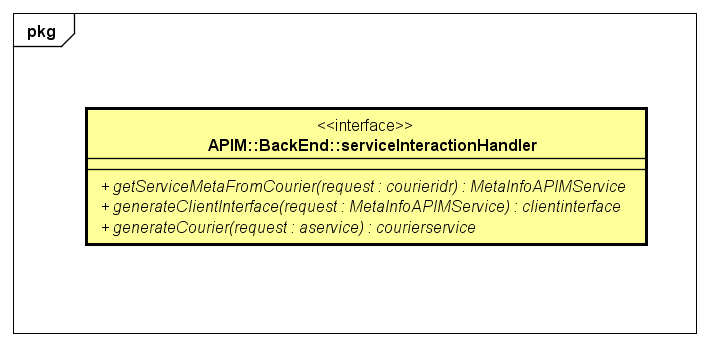
\includegraphics
	[width=0.7\linewidth]
	{images/APIM/BackEnd/Interfacce/ServiceInteractionHandlerInterface.png}
	\caption{Package APIM::BackEnd::ServiceInteractionHandlerInterface}
\end{figure}

\begin{itemize}
	\item \textbf{Descrizione:} L'interfaccia ServiceInteractionHandlerInterface contiene le operazioni riguardanti la gestione delle sessioni couriers e dei metadati dei microservizi. Viene utilizzata dal Gateway e da MicroservicesDB.
\end{itemize}

\subsection{APIMarket::Back-End::Gateway}

\subsubsection{Informazioni generali}

\begin{figure}[H]
	\centering
	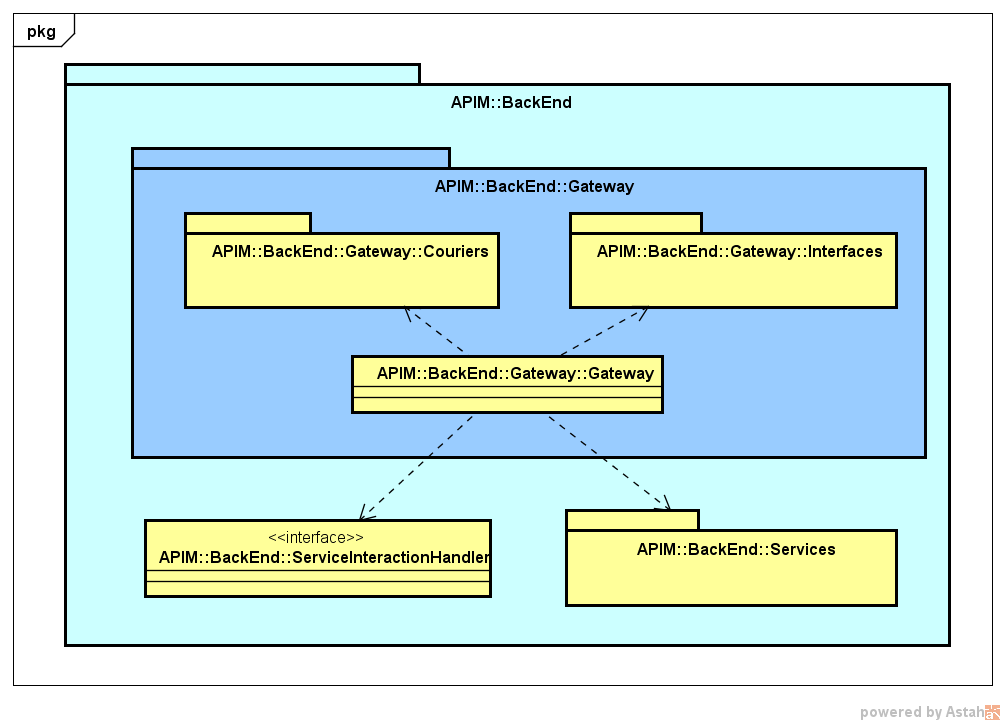
\includegraphics
	[width=0.7\linewidth]
	{UML/DiagrammiPackage/gateway.png}
	\caption{Package APIM::BackEnd::Gateway}
\end{figure}

\begin{itemize}
	\item \textbf{Descrizione:} Il package Gateway contiene le componenti del lato back-end dell'applicazione web.
	\item \textbf{Packages contenuti:}
	\begin{itemize}
		\item \textbf{Couriers:} package riguardante l'archiviazione delle sessioni couriers.
		\item \textbf{Interfaces:} package riguardante le interfacce necessarie alla classe Gateway.
	\end{itemize}
\end{itemize}

\subsubsection{Classi}

\paragraph{Gateway}
\begin{figure}[H]
	\centering
	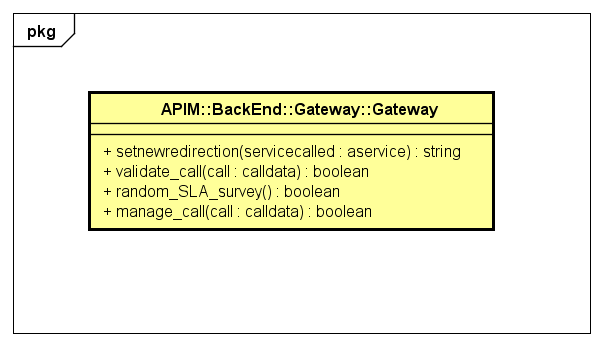
\includegraphics
	[width=0.7\linewidth]
	{images/APIM/BackEnd/Classi/apigateway.png}
	\caption{Package APIM::BackEnd::Gateway::Gateway}
\end{figure}

\begin{itemize}
	\item \textbf{Descrizione:} La classe Gateway genera le sessioni courier di ciascun microservizio presente in API Market al suo avvio, ed in seguito alla registrazione di un nuovo microservizio. Inoltre si occupa della verifica della chiamata al microservizio rispetto ai dati utente ed apikey, dei rilevamenti casuali di rispetto della SLA e della loro archiviazione, della redirection verso il microservizio e l'operazione desiderati.
	\item \textbf{Relazioni:}
		\begin{itemize}
			\item La classe Gateway implementa l'interfaccia RedirectorInterface;
			\item La classe Gateway utilizza le operazioni esposte dall'interfaccia ServiceInteractionHandler;
			\item La classe Gateway utilizza le operazione esposte dalle interfacce dei servizi di comunicazione con i database, presenti nel package Services;
			\item La classe Gateway genera le sessioni courier che vengono archiviate nel package Couriers.
		\end{itemize}
	\item \textbf{Operazioni:}
		\begin{itemize}
			\item \textbf{setnewredirection( aservice )( string ):} Genera il file di courier di un microservizio e ne imposta la redirection.
				\begin{description}
    				\item[\textbf{Parametri:}]
				\end{description}
				\begin{itemize}
					\item \textbf{aservice:} Dati del microservizio dal quale generare un file courier. 
				\end{itemize}
			\item \textbf{validate\_call( calldata )( bool ):} Valida la chiamata al microservizio, verificando utente e relativa apikey. 
				\begin{description}
    				\item[\textbf{Parametri:}]
				\end{description}
				\begin{itemize}
					\item \textbf{calldata:} Dati della chiamata al microservizio.
					\item \textbf{bool}.
				\end{itemize}
			\item \textbf{random\_SLA\_survey( void )( bool ):} Algoritmo casuale per scegliere se effettuare un sondaggio della SLA.
			\item \textbf{manage\_call( calldata )( bool ):} Gestisce la chiamata al microservizio.
				\begin{description}
    				\item[\textbf{Parametri:}]
				\end{description}
				\begin{itemize}
					\item \textbf{calldata:} Dati della chiamata al microservizio.
					\item \textbf{bool}.
				\end{itemize}
		\end{itemize}
\end{itemize}

\paragraph{ServiceInteractionHandler}
\begin{figure}[H]
	\centering
	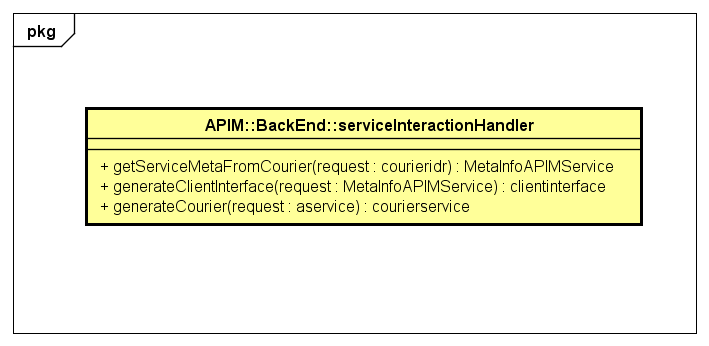
\includegraphics
	[width=0.7\linewidth]
	{images/APIM/BackEnd/Classi/ServiceInteractionHandler.png}
	\caption{Package APIM::BackEnd::Gateway::ServiceInteractionHandler}
\end{figure}

\begin{itemize}
	\item \textbf{Descrizione:} La classe ServiceInteractionHandler implementa l'interfaccia contenuta in APIM::BackEnd::Gateway::ServiceInteractionHandlerInterface.
	\item \textbf{Relazioni:}
		\begin{itemize}
			\item La classe ServiceInteractionHandler espone le proprie operazioni alla classe Gateway;
			\item La classe ServiceInteractionHandler espone le proprie operazioni alla classe Microservices\_db.
		\end{itemize}
	\item \textbf{Operazioni:}
		\begin{itemize}
			\item \textbf{GetServiceMetaFromCourier( courierdir )( MetaInfoAPIMService ):} Ricava da una courier i metadati del servizio, cioè tipi utilizzati ed operazioni fornite.
				\begin{description}
    				\item[\textbf{Parametri:}]
				\end{description}
				\begin{itemize}
					\item \textbf{courierdir:} Directory del file courier da cui estrarre le metainfo.
					\item \textbf{MetaInfoAPIMService:} Metadati di un microservizio registrato in API Market.
				\end{itemize}
			\item \textbf{generateClientInterface( MetaInfoAPIMService )( clientinterface ):} Genera l'interfaccia esposta al client del microservizio.
				\begin{description}
    				\item[\textbf{Parametri:}]
				\end{description}
				\begin{itemize}
					\item \textbf{MetaInfoAPIMService:} Metadati di un microservizio registrato in API Market.
					\item \textbf{clientinterface:} Rappresentazione come stringa dell'interfaccia esposta al client del microservizio.
				\end{itemize}
			\item \textbf{generateCourier( aservice )( courierservice ):} Genera la rappresentazione come stringa del file courier del microservizio.
				\begin{description}
    				\item[\textbf{Parametri:}]
				\end{description}
				\begin{itemize}
					\item \textbf{aservice:} Dati del microservizio dal quale generare un file courier.
					\item \textbf{courierservice:} Rappresentazione come stringa del file courier del microservizio.
				\end{itemize}
		\end{itemize}
\end{itemize}

\subsection{APIMarket::Back-End::Gateway::Couriers}

\subsubsection{Informazioni generali}

\begin{figure}[H]
	\centering
	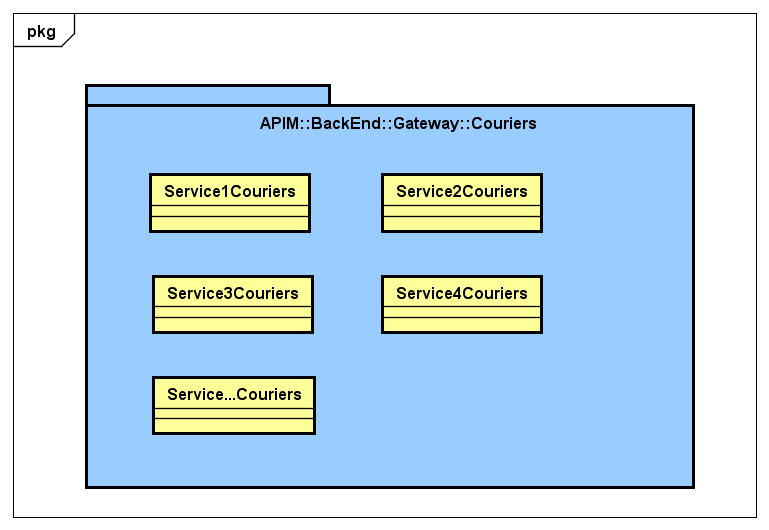
\includegraphics
	[width=0.7\linewidth]
	{UML/DiagrammiPackage/Couriers.png}
	\caption{Package APIM::BackEnd::Gateway::Couriers}
\end{figure}

\begin{itemize}
	\item \textbf{Descrizione:} Il package \textit{Couriers} archivia le sessioni couriers che si riferiscono ai singoli microservizi registrati su API Market. Le informazioni estese delle chiamate ai microservizi che esse contengono sono vitali per le classi Gateway e ServiceInteractionHandler. 
	Viene omessa la descrizione delle singole classi couriers in quanto il loro numero e la loro struttura dipende dai microservizi presenti in API Market.
\end{itemize}

\subsection{APIMarket::Back-End::Gateway::GatewayInterfaces}

\subsubsection{Informazioni generali}

\begin{figure}[H]
	\centering
	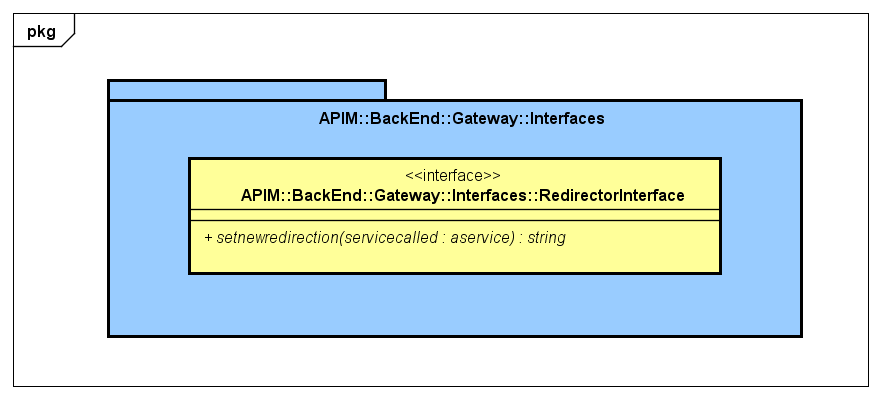
\includegraphics
	[width=0.7\linewidth]
	{UML/DiagrammiPackage/gatewayinterfaces.png}
	\caption{Package APIM::BackEnd::Gateway::GatewayInterfaces}
\end{figure}

\begin{itemize}
	\item \textbf{Descrizione:} Il package GatewayInterfaces contiene le interfacce necessarie al funzionamento del Gateway. In particolare si occupa delle attività di verifica, di gestione SLA e di redirection, trattando i dati riguardanti interfaccia ed operazione della chiamata ad un microservizio.
\end{itemize}

\subsubsection{Interfacce}

\paragraph{RedirectorInterface}
\begin{figure}[H]
	\centering
	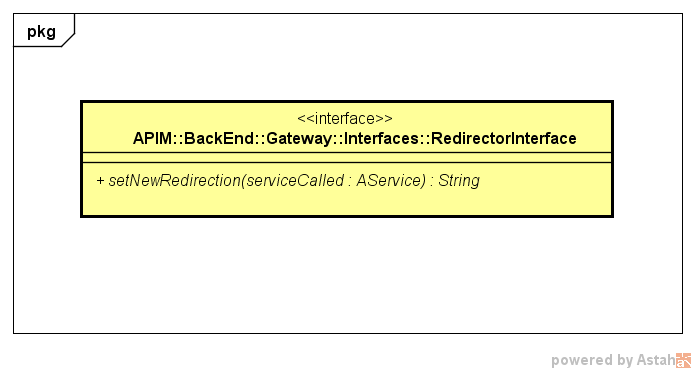
\includegraphics
	[width=0.7\linewidth]
	{images/APIM/BackEnd/Interfacce/RedirectorInterface.png}
	\caption{Package APIM::BackEnd::GatewayInterfaces/RedirectorInterface}
\end{figure}

\begin{itemize}
	\item \textbf{Descrizione:} L'interfaccia RedirectorInterface si occupa delle attività di redirection di una chiamata ad un microservizio. Sfruttando la classe ServiceInteractionHandler per generare una sessione courier, ne crea la classe Courier e le indirizza la redirection. Viene implementata dalla classe Gateway.
\end{itemize}

\subsection{APIMarket::Back-End::Services}

\subsubsection{Informazioni generali}

\begin{figure}[H]
	\centering
	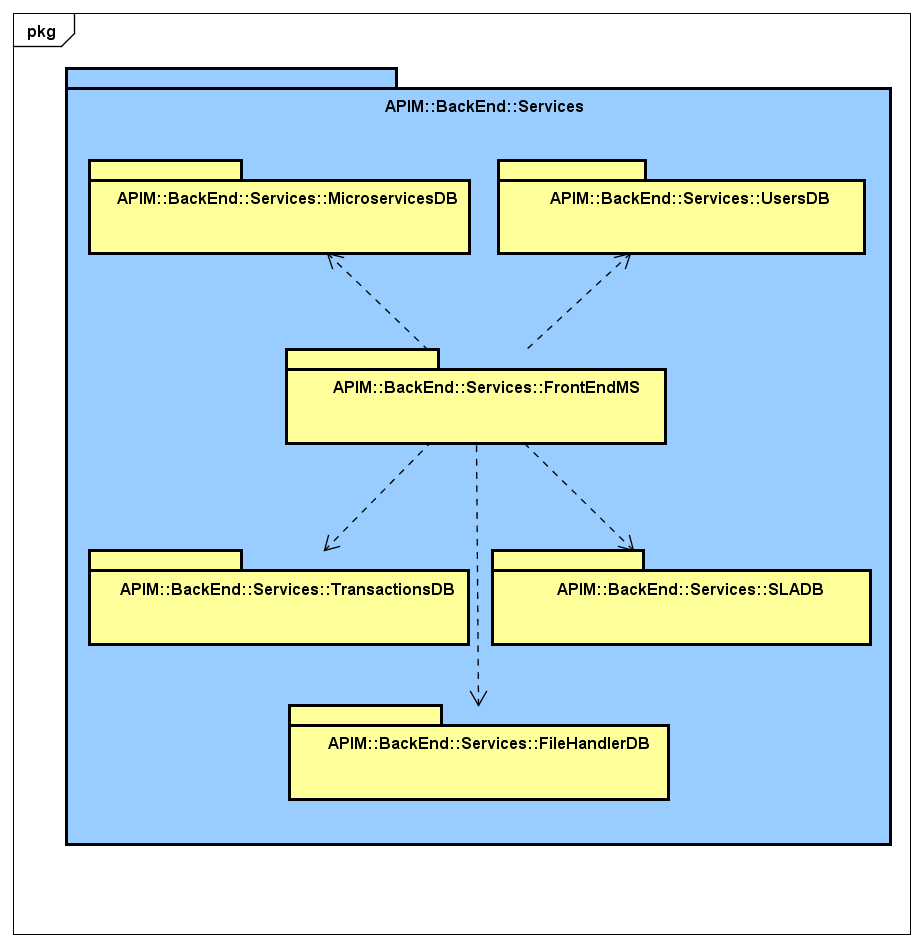
\includegraphics
	[width=0.7\linewidth]
	{UML/DiagrammiPackage/services.png}
	\caption{Package APIM::BackEnd::Services}
\end{figure}

\begin{itemize}
	\item \textbf{Descrizione:} Il package Services contiene le componenti per la comunicazione con i database di API Market.
	\item \textbf{Packages contenuti:}
	\begin{itemize}
		\item \textbf{MicroservicesDB:} package riguardante la comunicazione con il database dei microservizi registrati in API Market.
		\item \textbf{UsersDB:} package riguardante la comunicazione con il database degli utenti in API Market.
		\item \textbf{TransactionsDB:} package riguardante la comunicazione con il database delle transazioni in API Market.
		\item \textbf{SLADB:} package riguardante la comunicazione con il database della SLA in API Market.
		\item \textbf{FileHandlerDB:} package riguardante la comunicazione con il database dei file in API Market.
		\item \textbf{FrontEndMS:} package riguardante la comunicazione tra il front-end ed i vari database di API Market.
	\end{itemize}
\end{itemize}

\subsection{APIMarket::Back-End::Services::MicroservicesDB}

\subsubsection{Informazioni generali}

\begin{figure}[H]
	\centering
	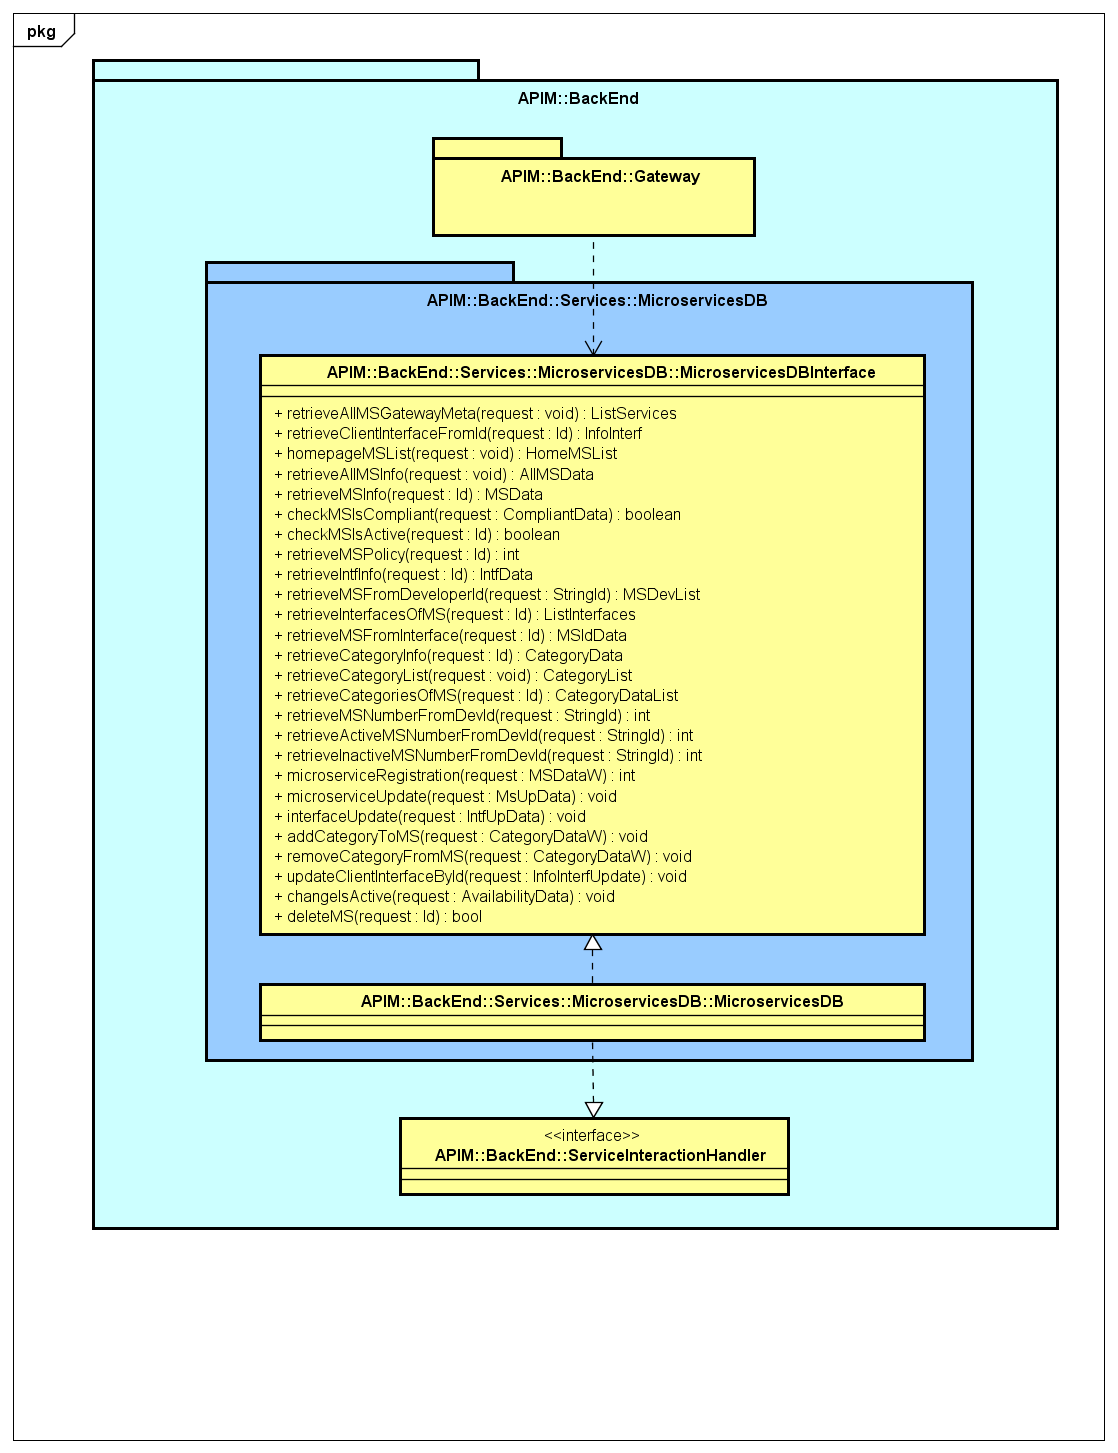
\includegraphics
	[width=0.7\linewidth]
	{UML/DiagrammiPackage/microservicesDB.png}
	\caption{Package APIM::BackEnd::Services::MicroservicesDB}
\end{figure}

\begin{itemize}
	\item \textbf{Descrizione:} Il package MicroservicesDB contiene le componenti per la comunicazione con i database dei microservizi di API Market.
\end{itemize}

\subsubsection{Interfacce}

\paragraph{Microservices\_dbInterface}
\begin{figure}[H]
	\centering
	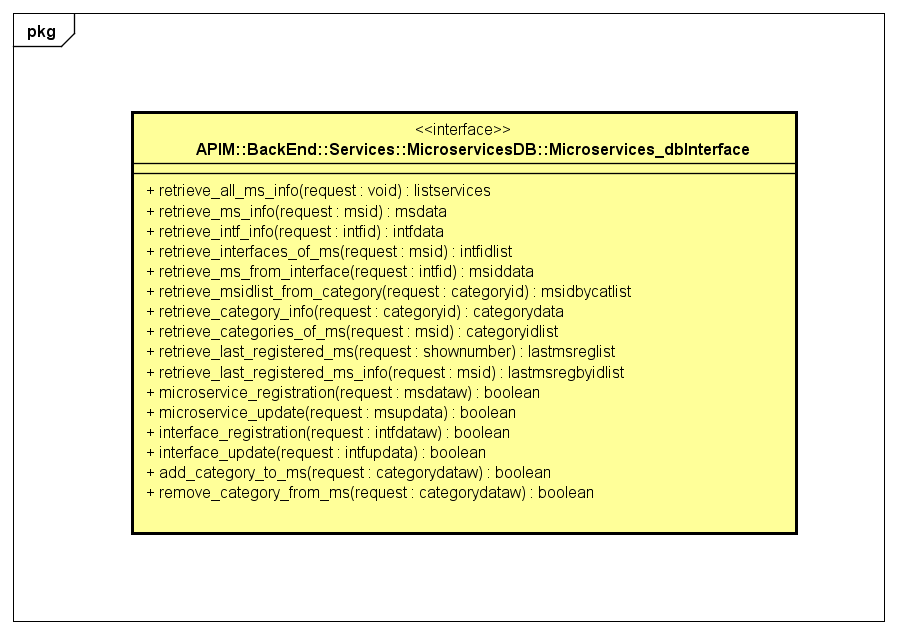
\includegraphics
	[width=0.7\linewidth]
	{images/APIM/BackEnd/Interfacce/microservices_dbInterface.png}
	\caption{Package APIM::BackEnd::Services::Microservices\_dbInterface}
\end{figure}

\begin{itemize}
	\item \textbf{Descrizione:} L'interfaccia Microservices\_dbInterface contiene le operazioni riguardanti lettura e scrittura dei dati dei microservizi, delle interfacce, delle categorie dei microservizi. Viene utilizzata da FrontendMS e dal Gateway.
\end{itemize}

\subsubsection{Classi}

\paragraph{Microservices\_db}
\begin{figure}[H]
	\centering
	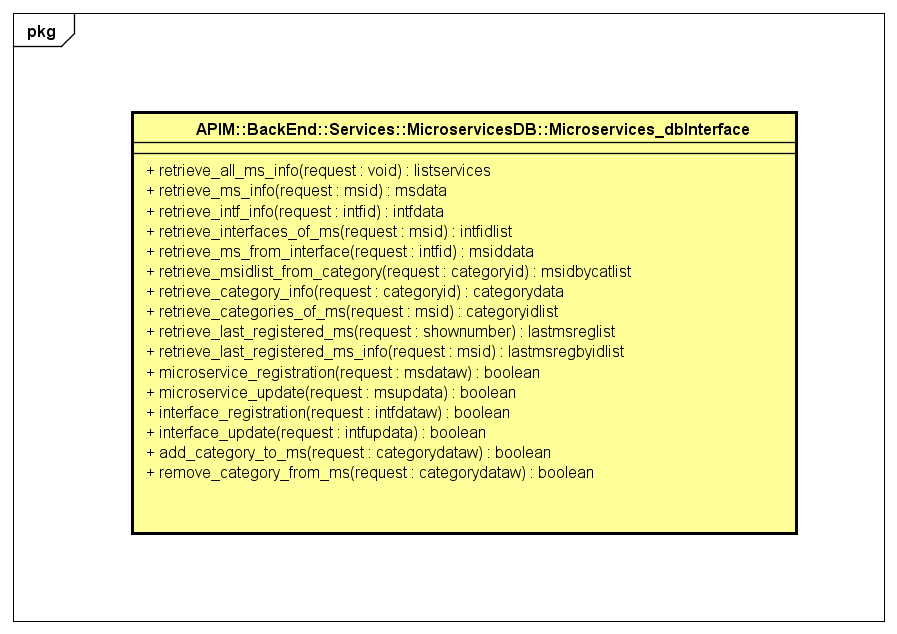
\includegraphics
	[width=0.7\linewidth]
	{images/APIM/BackEnd/Classi/microservices_db.png}
	\caption{Package APIM::BackEnd::Services::Microservices\_db}
\end{figure}

\begin{itemize}
	\item \textbf{Descrizione:} La classe Microservices\_db implementa l'interfaccia contenuta in APIM::BackEnd::Services::Microservices\_dbInterface.
	\item \textbf{Relazioni:}
		\begin{itemize}
			\item La classe Microservices\_db implementa l'interfaccia Microservices\_dbInterface;
			\item La classe Microservices\_db utilizza le operazioni esposte dall'interfaccia ServiceInteractionHandlerInterface;
			\item La classe Microservices\_db espone le proprie operazioni alla classe FrontendMS.
		\end{itemize}
	\item \textbf{Operazioni:}
		\begin{itemize}
		
			\item \textbf{retrieve\_all\_ms\_info( void )( listservices ):} Ricava le informazioni di ogni microservizio registrato in API Market.
				\begin{description}
    				\item[\textbf{Parametri:}]
				\end{description}
				\begin{itemize}
					\item \textbf{listservices:} Lista dei microservizi con relative informazioni.
				\end{itemize}
				
			\item \textbf{retrieve\_ms\_info( msid )( msdata ):} Ricava le informazioni del microservizio a partire dal suo id.
				\begin{description}
    				\item[\textbf{Parametri:}]
				\end{description}
				\begin{itemize}
					\item \textbf{msid:} Id del microservizio.
					\item \textbf{msdata:} Informazioni del microservizio.
				\end{itemize}
				
			\item \textbf{retrieve\_intf\_info( intfid )( intfdata ):} Ricava le informazioni dell'interfaccia a partire dal suo id.
				\begin{description}
    				\item[\textbf{Parametri:}]
				\end{description}
				\begin{itemize}
					\item \textbf{intfid:} Id dell'interfaccia.
					\item \textbf{intfdata:} Informazioni dell'interfaccia.
				\end{itemize}
				
			\item \textbf{retrieve\_interfaces\_of\_ms( msid )( intfidlist ):} Ricava gli id delle interfacce di un microservizio, a partire dal suo id.
				\begin{description}
    				\item[\textbf{Parametri:}]
				\end{description}
				\begin{itemize}
					\item \textbf{msid:} Id del microservizio.
					\item \textbf{intfidlist:} Lista degli id delle interfacce del microservizio.
				\end{itemize}
				
			\item \textbf{retrieve\_ms\_from\_interface( intfid )( msiddata ):} Ricava l'id del microservizio, a partire dall'id di una sua interfaccia.
				\begin{description}
    				\item[\textbf{Parametri:}]
				\end{description}
				\begin{itemize}
					\item \textbf{intfid:} Id dell'interfaccia.
					\item \textbf{msiddata:} Id del microservizio.
				\end{itemize}
				
			\item \textbf{retrieve\_msidlist\_from\_category( categoryid )( msidbycatlist ):} Ricava gli id dei microservizi appartenenti ad una categoria, a partire dall'id della categoria.
				\begin{description}
    				\item[\textbf{Parametri:}]
				\end{description}
				\begin{itemize}
					\item \textbf{categoryid:} Id della categoria.
					\item \textbf{msidbycatlist:} Lista degli id dei microservizi appartenenti alla categoria.
				\end{itemize}
				
			\item \textbf{retrieve\_category\_info( categoryid )( categorydata ):} Ricava le informazioni di una categoria, a partire dal suo id.
				\begin{description}
    				\item[\textbf{Parametri:}]
				\end{description}
				\begin{itemize}
					\item \textbf{categoryid:} Id della categoria.
					\item \textbf{categorydata:} Informazioni della categoria.
				\end{itemize}
				
			\item \textbf{retrieve\_categories\_of\_ms( msid )( categoryidlist ):} Ricava gli id delle categorie attribuite al microservizio, a partire dall'id del microservizio.
				\begin{description}
    				\item[\textbf{Parametri:}]
				\end{description}
				\begin{itemize}
					\item \textbf{msid:} Id del microservizio.
					\item \textbf{categoryidlist:} Lista degli id delle categorie attribuite al microservizio.
				\end{itemize}
				
			\item \textbf{retrieve\_last\_registered\_ms( shownumber )( lastmsreglist ):} Ricava un numero specificato dei microservizi registrati più recentemente su API Market.
				\begin{description}
    				\item[\textbf{Parametri:}]
				\end{description}
				\begin{itemize}
					\item \textbf{shownumber:} La lunghezza della lista massima dei microservizi registrati più recentemente su API Market.
					\item \textbf{lastmsreglist:} La lista dei microservizi registrati più recentemente su API Market con relative informazioni.
				\end{itemize}
				
			\item \textbf{retrieve\_last\_registered\_ms\_info( idms )( lastmsregbyidlist ):} Ricava Nome, IdDeveloper e Logo del microservizio, a partire dal suo id.
				\begin{description}
    				\item[\textbf{Parametri:}]
				\end{description}
				\begin{itemize}
					\item \textbf{msid:} Id del microservizio.
					\item \textbf{lastmsregbyidlist:} Name, IdDeveloper e Logo del microservizio.
				\end{itemize}
				
			\item \textbf{microservice\_registration( msdataw )( bool ):} Registra un nuovo microservizio nel database dei microservizi.
				\begin{description}
    				\item[\textbf{Parametri:}]
				\end{description}
				\begin{itemize}
					\item \textbf{msdataw:} Informazioni del nuovo microservizio.
					\item \textbf{bool}.
				\end{itemize}
				
			\item \textbf{microservice\_update( msupdata )( bool ):} Aggiorna le informazioni di un microservizio esistente nel database dei microservizi.
				\begin{description}
    				\item[\textbf{Parametri:}]
				\end{description}
				\begin{itemize}
					\item \textbf{msupdata:} Informazioni aggiornate di un microservizio esistente.
					\item \textbf{bool}.
				\end{itemize}
				
			\item \textbf{interface\_registration( intfdataw )( bool ):} Registra una nuova interfaccia di un microservizio esistente nel database dei microservizi .
				\begin{description}
    				\item[\textbf{Parametri:}]
				\end{description}
				\begin{itemize}
					\item \textbf{intfdataw:} Informazioni della nuova interfaccia.
					\item \textbf{bool}.
				\end{itemize}
				
			\item \textbf{interface\_update( intfupdata )( bool):} Aggiorna le informazioni di una interfaccia esistente nel database dei microservizi.
				\begin{description}
    				\item[\textbf{Parametri:}]
				\end{description}
				\begin{itemize}
					\item \textbf{intfupdata:} Informazioni aggiornate di una interfaccia esistente.
					\item \textbf{bool}.
				\end{itemize}
				
			\item \textbf{add\_category\_to\_ms( categorydataw )( bool ):} Attribuisce una categoria ad un microservizio.
				\begin{description}
    				\item[\textbf{Parametri:}]
				\end{description}
				\begin{itemize}
					\item \textbf{categorydataw:} Id del microservizio e della categoria da attribuirgli.
					\item \textbf{bool}.
				\end{itemize}
				
			\item \textbf{remove\_category\_from\_ms( categorydataw )( bool ):} Rimuove una categoria da un microservizio.
				\begin{description}
    				\item[\textbf{Parametri:}]
				\end{description}
				\begin{itemize}
					\item \textbf{categorydataw:} Id del microservizio e della categoria da rimuovergli.
					\item \textbf{bool}.
				\end{itemize}
	
		\end{itemize}
\end{itemize}

\subsection{APIMarket::Back-End::Services::UsersDB}

\subsubsection{Informazioni generali}

\begin{figure}[H]
	\centering
	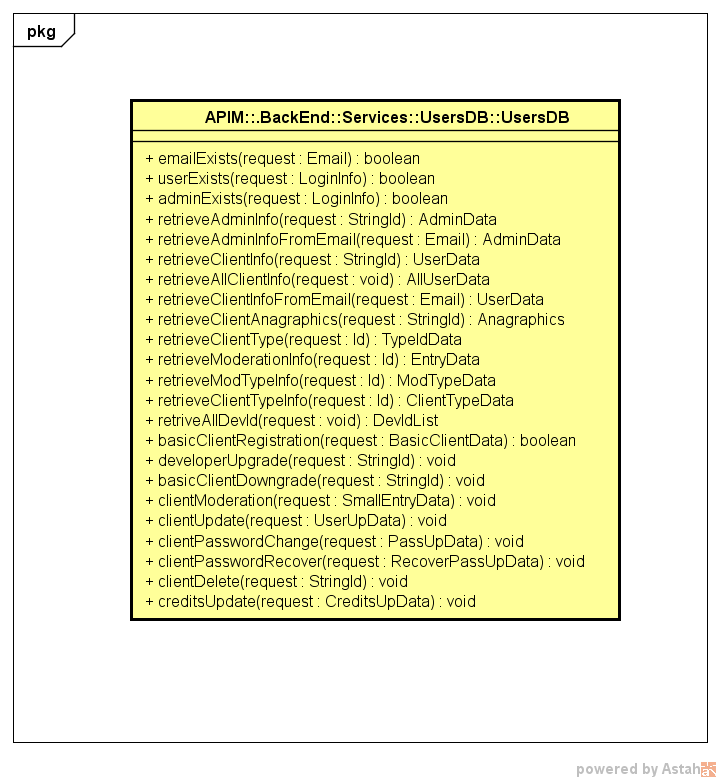
\includegraphics
	[width=0.7\linewidth]
	{UML/DiagrammiPackage/usersDB.png}
	\caption{Package APIM::BackEnd::Services::UsersDB}
\end{figure}

\begin{itemize}
	\item \textbf{Descrizione:} Il package \textit{UsersDB} contiene le componenti per la comunicazione con il database degli utenti di API Market.
\end{itemize}

\subsubsection{Interfacce}

\paragraph{UsersDBInterface}
\begin{figure}[H]
	\centering
	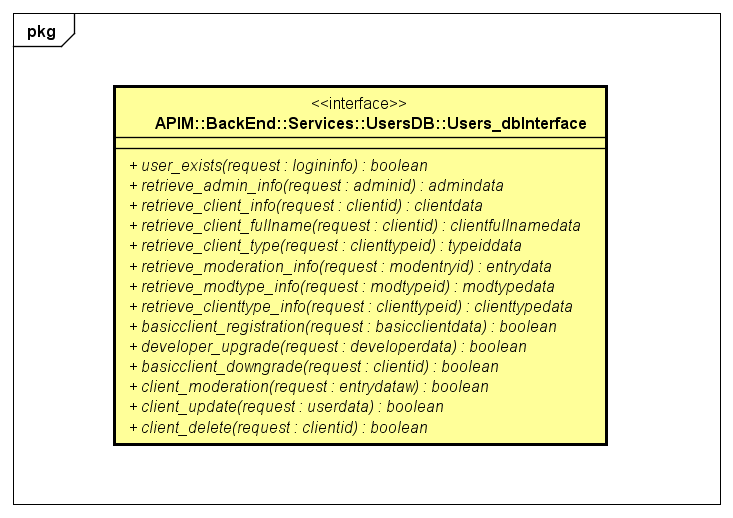
\includegraphics
	[width=0.7\linewidth]
	{images/APIM/BackEnd/Interfacce/users_dbInterface.png}
	\caption{Package APIM::BackEnd::Services::Users\_dbInterface}
\end{figure}

\begin{itemize}
	\item \textbf{Descrizione:} L'interfaccia Users\_dbInterface contiene le operazioni riguardanti lettura e scrittura dei dati degli utenti (sia admin che clienti), dei tipi di cliente, delle moderazioni attuate, dei tipi di moderazione. Viene utilizzata da FrontendMS e dal Gateway.
\end{itemize}

\subsubsection{Classi}

\paragraph{Users\_db}
\begin{figure}[H]
	\centering
	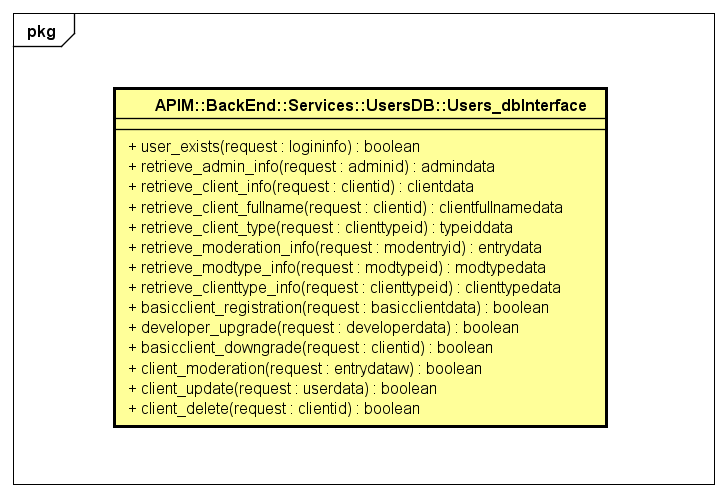
\includegraphics
	[width=0.7\linewidth]
	{images/APIM/BackEnd/Classi/users_db.png}
	\caption{Package APIM::BackEnd::Services::Users\_db}
\end{figure}

\begin{itemize}
	\item \textbf{Descrizione:} La classe Users\_db implementa l'interfaccia contenuta in APIM::BackEnd::Services::Users\_dbInterface.
	\item \textbf{Relazioni:}
		\begin{itemize}
			\item La classe Users\_db implementa l'interfaccia Users\_dbInterface;
			\item La classe Users\_db espone le proprie operazioni alla classe FrontendMS.
		\end{itemize}
	\item \textbf{Operazioni:}
		\begin{itemize}
		
			\item \textbf{user\_exists( logininfo )( bool ):} Controlla se il cliente esista nel database utenti.
				\begin{description}
    				\item[\textbf{Parametri:}]
				\end{description}
				\begin{itemize}
					\item \textbf{logininfo:} Email ed Password del cliente.
					\item \textbf{bool}.
				\end{itemize}
				
			\item \textbf{retrieve\_admin\_info( adminid )( admindata ):} Ricava le informazioni dell'admin, a partire dal suo id.
				\begin{description}
    				\item[\textbf{Parametri:}]
				\end{description}
				\begin{itemize}
					\item \textbf{adminid:} Id dell'admin.
					\item \textbf{admindata:} Informazioni dell'admin.
				\end{itemize}
				
			\item \textbf{retrieve\_client\_info( clientid )( clientdata ):} Ricava le informazioni del cliente, a partire dal suo id.
				\begin{description}
    				\item[\textbf{Parametri:}]
				\end{description}
				\begin{itemize}
					\item \textbf{clientid:} Id del cliente.
					\item \textbf{clientdata:} Informazioni del cliente.
				\end{itemize}
				
			\item \textbf{retrieve\_client\_fullname( clientid )( clientfullnamedata ):} Ricava Name e Surname del client, a partire dal suo id.
				\begin{description}
    				\item[\textbf{Parametri:}]
				\end{description}
				\begin{itemize}
					\item \textbf{clientid:} Id del cliente.
					\item \textbf{clientfullnamedata:} Name e Surname del cliente.
				\end{itemize}
				
			\item \textbf{retrieve\_client\_type( clientid )( typeiddata ):} Ricava il tipo di account del cliente, a partire dal suo id.
				\begin{description}
    				\item[\textbf{Parametri:}]
				\end{description}
				\begin{itemize}
					\item \textbf{clientid:} Id del cliente.
					\item \textbf{typeiddata:} Id del tipo di account del cliente.
				\end{itemize}
			
			\item \textbf{retrieve\_moderation\_info( modentryid )( entrydata ):} Ricava le informazioni della moderazione, a partire dal suo id.
				\begin{description}
    				\item[\textbf{Parametri:}]
				\end{description}
				\begin{itemize}
					\item \textbf{modentryid:} Id della moderazione.
					\item \textbf{entrydata:} Informazioni della moderazione.
				\end{itemize}
				
			\item \textbf{retrieve\_modtype\_info( modtypeid )( modtypedata ):} Ricava le informazioni del tipo di moderazione, a partire dal suo id.
				\begin{description}
    				\item[\textbf{Parametri:}]
				\end{description}
				\begin{itemize}
					\item \textbf{modtypeid:} Id del tipo di moderazione.
					\item \textbf{modtypedata:} Informazioni del tipo di moderazione.
				\end{itemize}
				
			\item \textbf{retrieve\_clienttype\_info( clienttypeid )( clienttypedata ):} Ricava le informazioni del tipo di account del cliente, a partire dal suo id.
				\begin{description}
    				\item[\textbf{Parametri:}]
				\end{description}
				\begin{itemize}
					\item \textbf{clienttypeid:} Id del tipo di account del cliente.
					\item \textbf{clienttypedata:} Informazioni del tipo di account del cliente.
				\end{itemize}
				
			\item \textbf{basicclient\_registration( basicclientdata )( bool ):} Registra un nuovo account cliente di tipo base.
				\begin{description}
    				\item[\textbf{Parametri:}]
				\end{description}
				\begin{itemize}
					\item \textbf{basicclientdata:} Informazioni del nuovo cliente.
					\item \textbf{bool}.
				\end{itemize}
				
			\item \textbf{developer\_upgrade( developerdata )( bool ):} Effettua l'upgrade ad account sviluppatore di un cliente.
				\begin{description}
    				\item[\textbf{Parametri:}]
				\end{description}
				\begin{itemize}
					\item \textbf{developerdata:} Informazioni dei campi aggiuntivi da sviluppatore.
					\item \textbf{bool}.
				\end{itemize}
				
			\item \textbf{basicclient\_downgrade( clientid )( bool ):} Effettua il downgrade ad account base di un cliente sviluppatore.
				\begin{description}
    				\item[\textbf{Parametri:}]
				\end{description}
				\begin{itemize}
					\item \textbf{clientid:} Id del cliente.
					\item \textbf{bool}.
				\end{itemize}
				
			\item \textbf{client\_moderation( entrydataw )( bool ):} Inserisce una nuova moderazione nel database degli utenti.
				\begin{description}
    				\item[\textbf{Parametri:}]
				\end{description}
				\begin{itemize}
					\item \textbf{entrydataw:} Informazioni della nuova moderazione.
					\item \textbf{bool}.
				\end{itemize}
				
			\item \textbf{client\_update( userdata )( bool ):} Aggiorna le informazioni di un cliente.
				\begin{description}
    				\item[\textbf{Parametri:}]
				\end{description}
				\begin{itemize}
					\item \textbf{userdata:} Informazioni aggiornate del cliente.
					\item \textbf{bool}.
				\end{itemize}
				
			\item \textbf{client\_delete( clientid )( bool ):} Elimina un cliente da API Market.
				\begin{description}
    				\item[\textbf{Parametri:}]
				\end{description}
				\begin{itemize}
					\item \textbf{clientid:} Id del cliente.
					\item \textbf{bool}.
				\end{itemize}
					
		\end{itemize}
\end{itemize}

\subsection{APIMarket::Back-End::Services::TransactionsDB}

\subsubsection{Informazioni generali}

\begin{figure}[H]
	\centering
	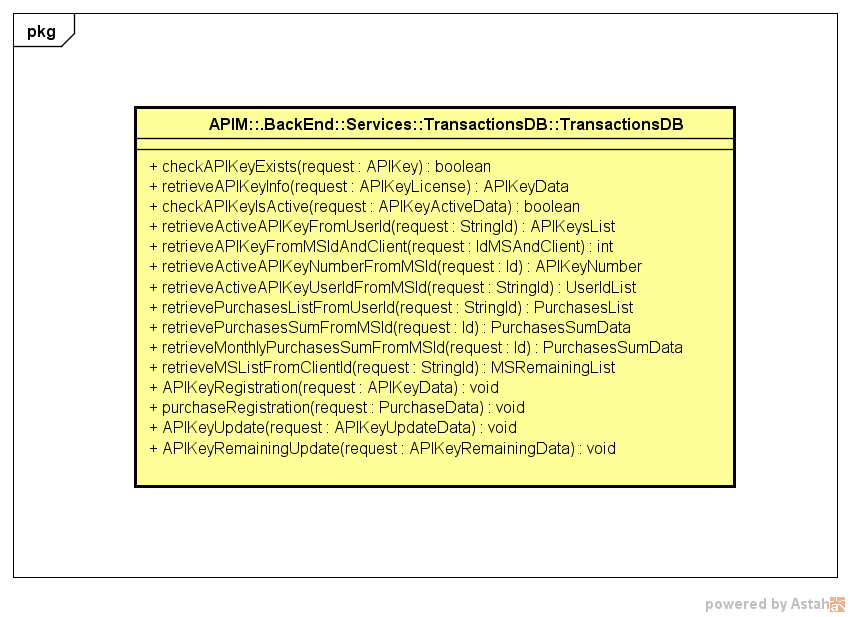
\includegraphics
	[width=0.7\linewidth]
	{UML/DiagrammiPackage/transactionsDB.png}
	\caption{Package APIM::BackEnd::Services::TransactionsDB}
\end{figure}

\begin{itemize}
	\item \textbf{Descrizione:} Il package \textit{TransactionsDB} contiene le componenti per la comunicazione con il database delle transazioni di API Market.
\end{itemize}

\subsubsection{Interfacce}

\paragraph{Transactions\_dbInterface}
\begin{figure}[H]
	\centering
	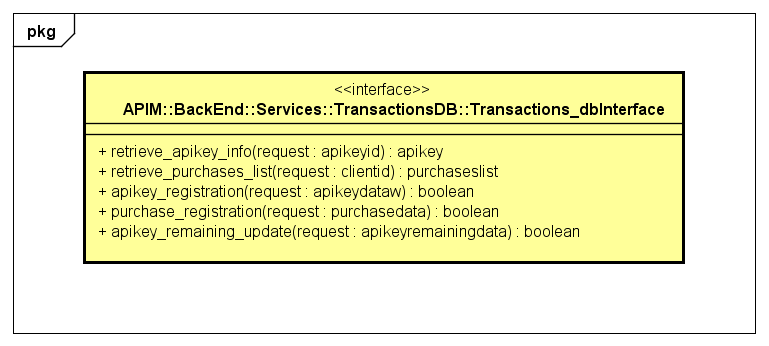
\includegraphics
	[width=0.7\linewidth]
	{images/APIM/BackEnd/Interfacce/transactions_dbInterface.png}
	\caption{Package APIM::BackEnd::Services::Transactions\_dbInterface}
\end{figure}

\begin{itemize}
	\item \textbf{Descrizione:} L'interfaccia Transactions\_dbInterface contiene le operazioni riguardanti lettura e scrittura dei dati delle apikey, degli acquisti. Viene utilizzata da FrontendMS e dal Gateway.
\end{itemize}

\subsubsection{Classi}

\paragraph{Transactions\_db}
\begin{figure}[H]
	\centering
	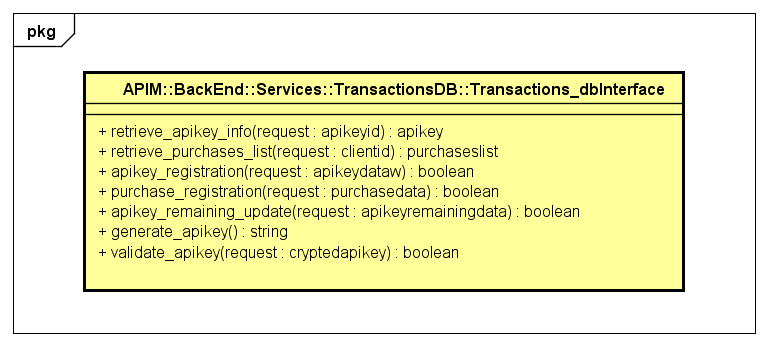
\includegraphics
	[width=0.7\linewidth]
	{images/APIM/BackEnd/Classi/transactions_db.png}
	\caption{Package APIM::BackEnd::Services::Transactions\_db}
\end{figure}

\begin{itemize}
	\item \textbf{Descrizione:} La classe Transactions\_db implementa l'interfaccia contenuta in APIM::BackEnd::Services::Transactions\_dbInterface.
	\item \textbf{Relazioni:}
		\begin{itemize}
			\item La classe Transactions\_db implementa l'interfaccia Transactions\_dbInterface;
			\item La classe Transactions\_db espone le proprie operazioni alla classe FrontendMS.
		\end{itemize}
	\item \textbf{Operazioni:}
		\begin{itemize}
		
			\item \textbf{retrieve\_apikey\_info( apikeyid )( apikey ):} Ricava le informazioni dell'apikey, a partire dal suo id.
				\begin{description}
    				\item[\textbf{Parametri:}]
				\end{description}
				\begin{itemize}
					\item \textbf{apikeyid:} Id dell'apikey.
					\item \textbf{apikey:} Informazioni dell'apikey.
				\end{itemize}
				
			\item \textbf{retrieve\_purchases\_list( clientid )( purchaseslist ):} Ricava la lista con relative informazioni delle transazioni del cliente, a partire dal suo id.
				\begin{description}
    				\item[\textbf{Parametri:}]
				\end{description}
				\begin{itemize}
					\item \textbf{clientid:} Id del cliente.
					\item \textbf{purchaseslist:} Lista delle transazioni del cliente con relative informazioni.
				\end{itemize}
				
			\item \textbf{apikey\_registration( apikeydataw )( bool ):} Registra una nuova apikey nel database delle transazioni.
				\begin{description}
    				\item[\textbf{Parametri:}]
				\end{description}
				\begin{itemize}
					\item \textbf{apikeydataw:} Informazioni della nuova apikey.
					\item \textbf{bool}.
				\end{itemize}
				
			\item \textbf{purchase\_registration( purchasedata )( bool ):} Inserisce una nuova transazione nel database delle transazioni.
				\begin{description}
    				\item[\textbf{Parametri:}]
				\end{description}
				\begin{itemize}
					\item \textbf{purchasedata:} Informazioni della nuova transazione.
					\item \textbf{bool}.
				\end{itemize}
				
			\item \textbf{apikey\_remaining\_update( apikeyremainingdata )( bool ):} Aggiorna il Remaining della apikey, a partire dal suo id e dal valore del cambiamento.
				\begin{description}
    				\item[\textbf{Parametri:}]
				\end{description}
				\begin{itemize}
					\item \textbf{apikeyremainingdata:} Id dell'apikey e valore del cambiamento.
					\item \textbf{bool}.
				\end{itemize}
				
		\end{itemize}
\end{itemize}

\subsection{APIMarket::Back-End::Services::SLADB}

\subsubsection{Informazioni generali}

\begin{figure}[H]
	\centering
	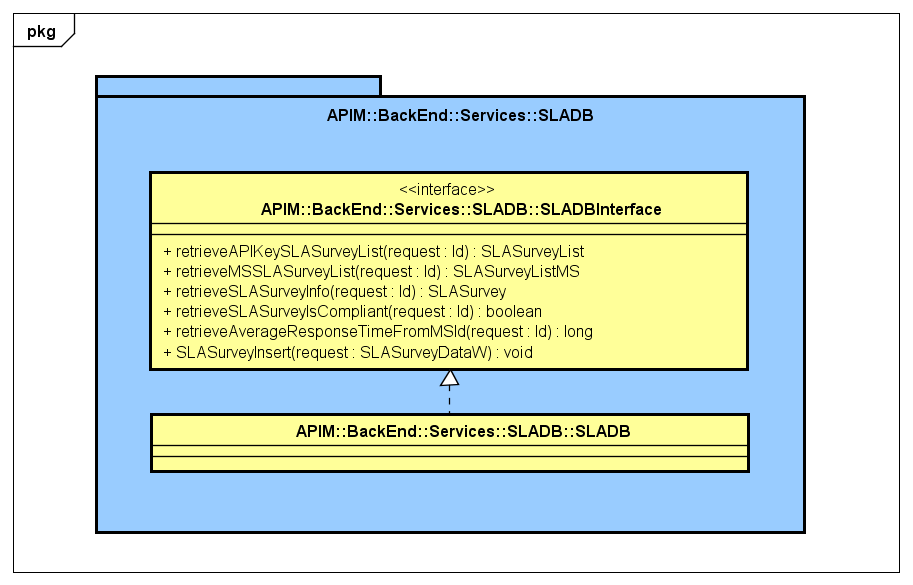
\includegraphics
	[width=0.7\linewidth]
	{UML/DiagrammiPackage/SLADB.png}
	\caption{Package APIM::BackEnd::Services::SLADB}
\end{figure}

\begin{itemize}
	\item \textbf{Descrizione:} Il package \textit{SLADB} contiene le componenti per la comunicazione con il database della SLA di API Market.
\end{itemize}

\subsubsection{Interfacce}

\paragraph{Sla\_dbInterface}
\begin{figure}[H]
	\centering
	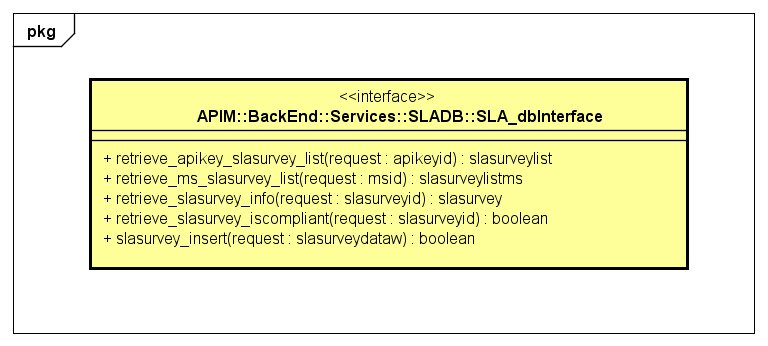
\includegraphics
	[width=0.7\linewidth]
	{images/APIM/BackEnd/Interfacce/sla_dbInterface.png}
	\caption{Package APIM::BackEnd::Services::Sla\_dbInterface}
\end{figure}

\begin{itemize}
	\item \textbf{Descrizione:} L'interfaccia Sla\_dbInterface contiene le operazioni riguardanti lettura e scrittura dei dati dei sondaggi SLA. Viene utilizzata da FrontendMS e dal Gateway.
\end{itemize}

\subsubsection{Classi}

\paragraph{Sla\_db}
\begin{figure}[H]
	\centering
	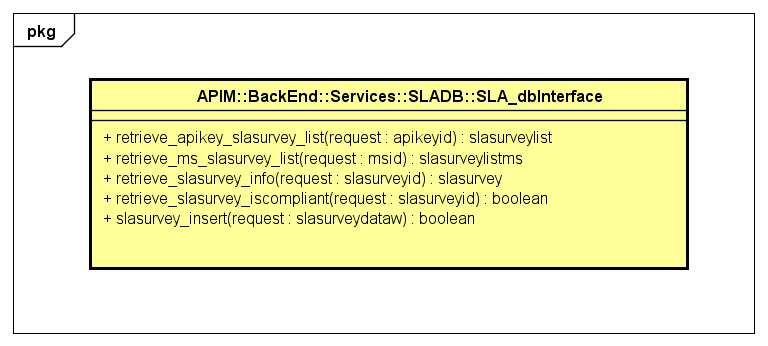
\includegraphics
	[width=0.7\linewidth]
	{images/APIM/BackEnd/Classi/sla_db.png}
	\caption{Package APIM::BackEnd::Services::Sla\_db}
\end{figure}

\begin{itemize}
	\item \textbf{Descrizione:} La classe Sla\_db implementa l'interfaccia contenuta in APIM::BackEnd::Services::Sla\_dbInterface.
	\item \textbf{Relazioni:}
		\begin{itemize}
			\item La classe Sla\_db implementa l'interfaccia Sla\_dbInterface;
			\item La classe Sla\_db espone le proprie operazioni alla classe FrontendMS.
		\end{itemize}
	\item \textbf{Operazioni:}
		\begin{itemize}
		
			\item \textbf{retrieve\_apikey\_slasurvey\_list( apikeyid )( slasurveylist ):} Ricava la lista dei sondaggi SLA dell'apikey con relative informazioni, a partire dall'id dell'apikey.
				\begin{description}
    				\item[\textbf{Parametri:}]
				\end{description}
				\begin{itemize}
					\item \textbf{apikeyid:} Id dell'apikey.
					\item \textbf{slasurveylist:} Lista dei sondaggi SLA con relative informazioni.
				\end{itemize}
				
			\item \textbf{retrieve\_ms\_slasurvey\_list( msid )( slasurveylistms ):} Ricava la lista dei sondaggi SLA del microservizio con relative informazioni, a partire dall'id del microservizio.
				\begin{description}
    				\item[\textbf{Parametri:}]
				\end{description}
				\begin{itemize}
					\item \textbf{msid:} Id del microservizio.
					\item \textbf{slasurveylistms:} Lista dei sondaggi SLA con relative informazioni.
				\end{itemize}
				
			\item \textbf{retrieve\_slasurvey\_info( slasurveyid )( slasurvey ):} Ricava le informazioni del sondaggio SLA, a partire dal suo id.
				\begin{description}
    				\item[\textbf{Parametri:}]
				\end{description}
				\begin{itemize}
					\item \textbf{slasurveyid:} Id del sondaggio SLA.
					\item \textbf{slasurvey:} Informazioni del sondaggio SLA.
				\end{itemize}
				
			\item \textbf{retrieve\_slasurvey\_iscompliant( slasurveyid )( bool ):} Ricava IsCompliant del sondaggio SLA, a partire dal suo id.
				\begin{description}
    				\item[\textbf{Parametri:}]
				\end{description}
				\begin{itemize}
					\item \textbf{slasurveyid:} Id del sondaggio SLA.
					\item \textbf{bool}.
				\end{itemize}
				
			\item \textbf{slasurvey\_insert( slasurveydataw )( bool ):} Inserisce un nuovo sondaggio SLA nel database della SLA.
				\begin{description}
    				\item[\textbf{Parametri:}]
				\end{description}
				\begin{itemize}
					\item \textbf{slasurveydataw:} Informazioni del nuovo sondaggio SLA.
					\item \textbf{bool}.
				\end{itemize}
				
		\end{itemize}
\end{itemize}

\subsection{APIMarket::Back-End::Services::FilehandlerDB}

\subsubsection{Informazioni generali}

\begin{figure}[H]
	\centering
	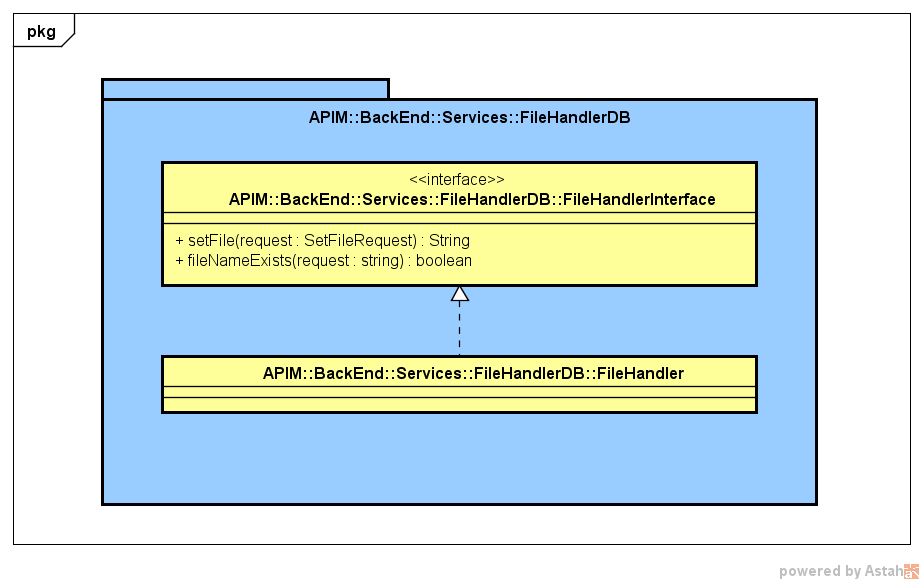
\includegraphics
	[width=0.7\linewidth]
	{UML/DiagrammiPackage/filehandlerDB.png}
	\caption{Package APIM::BackEnd::Services::FilehandlerDB}
\end{figure}

\begin{itemize}
	\item \textbf{Descrizione:} Il package FilehandlerDB contiene le componenti per la comunicazione con il database dei file di API Market.
\end{itemize}

\subsubsection{Interfacce}

\paragraph{Filehandler\_dbInterface}
\begin{figure}[H]
	\centering
	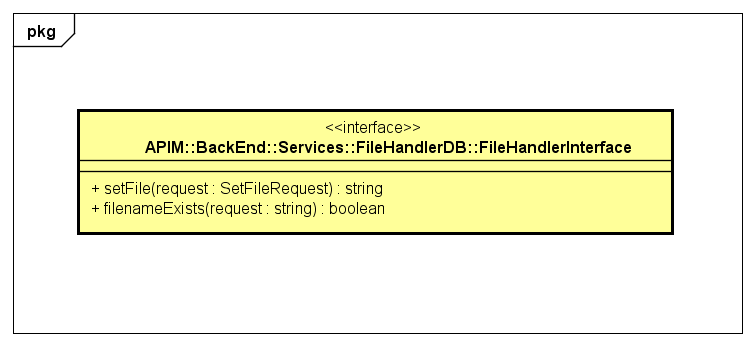
\includegraphics
	[width=0.7\linewidth]
	{images/APIM/BackEnd/Interfacce/filehandler_dbInterface.png}
	\caption{Package APIM::BackEnd::Services::Filehandler\_dbInterface}
\end{figure}

\begin{itemize}
	\item \textbf{Descrizione:} L'interfaccia Filehandler\_dbInterface contiene le operazioni riguardanti lettura e scrittura dei dati dei file. Viene utilizzata da FrontendMS e dal Gateway.
\end{itemize}

\subsubsection{Classi}

\paragraph{Filehandler\_db}
\begin{figure}[H]
	\centering
	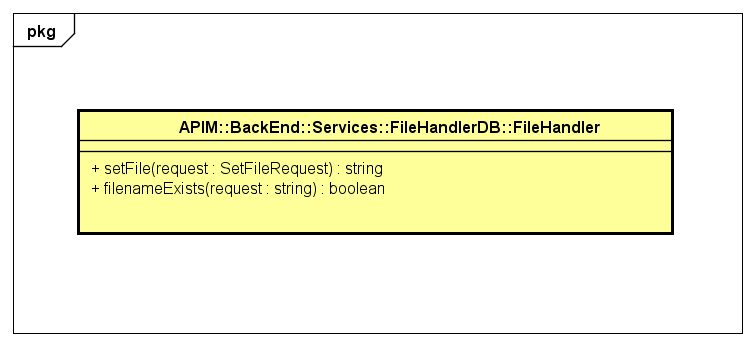
\includegraphics
	[width=0.7\linewidth]
	{images/APIM/BackEnd/Classi/filehandler_db.png}
	\caption{Package APIM::BackEnd::Services::Filehandler\_db}
\end{figure}

\begin{itemize}
	\item \textbf{Descrizione:} La classe Filehandler\_db implementa l'interfaccia contenuta in APIM::BackEnd::Services::Filehandler\_dbInterface.
	\item \textbf{Relazioni:}
		\begin{itemize}
			\item La classe Filehandler\_db implementa l'interfaccia Filehandler\_dbInterface;
			\item La classe Filehandler\_db espone le proprie operazioni alla classe FrontendMS.
		\end{itemize}
	\item \textbf{Operazioni:}
		\begin{itemize}
		
			\item \textbf{setFile( SetFileRequest )( string ):} Archivia il file, se non è già presente nell'archivio, salvandolo con un nome univoco e ricava l'uri corrispondente.
				\begin{description}
    				\item[\textbf{Parametri:}]
				\end{description}
				\begin{itemize}
					\item \textbf{SetFileRequest:} Informazioni del file.
					\item \textbf{string}.
				\end{itemize}
				
			\item \textbf{filenameExists( string )( bool ):} Controlla se nel database dei file esista un file con il nome specificato.
				\begin{description}
    				\item[\textbf{Parametri:}]
				\end{description}
				\begin{itemize}
					\item \textbf{string}.
					\item \textbf{bool}.
				\end{itemize}
				
		\end{itemize}
\end{itemize}